\documentclass{article}
\usepackage[utf8]{inputenc}
\usepackage{graphicx}

\title{Brief Overview of SmartFin Version 3 Scheduler Implementation}
\author{Antara Chugh}
\date{Summer 2024}

\begin{document}

\maketitle

\section{Background on the SmartFin System}

We are working to design a scheduler for multiple sensors running at various frequencies and durations on a single threaded system that can only run one sensor at a time. The hardware thus restricts the schedule to be non-pre-emptitive: we cannot stop or pause a sensor A from running if another sensor B must run during the duration sensor A is collecting data. From now on, we’ll refer to each sensor as a repeating, periodic task that must run for x amount of time every y seconds. \newline


\title{Table 1: Mean \& Standard Deviation Runtime of SmartFin Sensors}
\newline



\begin{tabular}{c|c}
\hspace{-3 cm}
\begin{tabular}{| l | l | l | l | l |}
\hline
Sensor & Mean (ms) & Standard Deviation (ms) & Mean + 3 Std (ms) & Frequency \\
\hline
Temperature & 0.873 & 0.002 & 0.881 & 1 Hz \\
\hline
Accelerometer & 5.244 & 0.004 & 5.255 & 30-300 Hz \\
\hline
Gyroscope & 5.209 & 0.003 & 5.218 & 30-300 Hz \\
\hline
Magnetometer & 5.212 & 0.004 & 5.221 & 30-300 Hz \\
\hline
GPS (reading no valid location) & 0.1443 & 0.022 & 0.2103 & 1 Hz \\
\hline
Wet/Dry Sensor & 1.02 & 0.002 & 1.025 & 1 Hz \\
\hline

\end{tabular}

\end{tabular}





\section{Scheduler Requirements}
\begin{itemize}
    \item Non-preemptive 
    \item Maintain the frequency of each task (consistent data  sampling) 
    \item Delay or “shift” a sampling schedule of a task rather than having a singular task out of place, as that data point would then not be usable 
    \item Have minimal “shifts”; if priority is implemented, then minimize the “shifts” of each task by priority
\end{itemize}

The most important quality for our schedule is that it maintains the frequency of each task as much as possible in order to maximize the percentage of samples that can be used for further data processing. For our system, a delay can better be defined as a shift of the sampling sequence: If task A was scheduled to run every 5 seconds starting at time 0, but a delay in the system prevented A from running at t=10 seconds and instead ran at t=12 seconds, we say that the sampling sequence of A was shifted, or delayed by 2 seconds. A will now run every 5 seconds starting from t=12, and thus will run again at t=17 seconds. Our scheduler thus seeks to minimize the amount of these “shifts” in the system. As noted above, we prefer these “shifts” over delays to singular tasks, as that would violate the consistent sample rate we hope to achieve. 


In addition, minimizing the number of shifts in the sampling sequence may be more important for some tasks than others. For example, it is more important for data processing that the inertial measurement unit is sampled at a constant rate with little to no shifts than the GPS. Thus, there is incentive to introduce some method of maintaining priority of the tasks. This works best for systems with a small number of tasks that run for relatively short durations and have relatively long time between runs. For schedulers that are more overloaded, this notion of priority may shift the sampling schedules of low priority tasks too drastically, worst case stopping them from running at all. In this case, priority may have to be implemented differently, perhaps with a max shift time enforcement (no task can be shifted more than x seconds) or having no priority in the system at all. 

Another factor to note is that the exact amount of time the system will run is variable, as surfers spend variable amounts of time in the water. 

\section{Previous Works}
There has been much work already done on non-preemptive scheduler algorithms. \newline

Greedy algorithms are those based on making the most locally optimal decision. Earliest deadline first and earliest job finished are examples of greedy algorithms used for creating schedules with a single compute source and multiple tasks with potentially overlapping times (Karger 1997). \newline

Earliest Deadline First is a greedy algorithm for soft real time systems, which allow for tasks to be late (Karger 1997). It provides the optimal solution to minimizing lateness in the system. It schedules tasks by ascending deadlines, scheduling those with the earliest deadline first (as implied by its name).Though we wish to also minimize delays in the system, we would prefer to delay a task and all subsequent occurrences of that task to maintain a consistent sampling rate over having a task delayed and that data point rendered as not usable. Thus, earliest deadline first is not a feasible algorithm, as it cannot guarantee consistent periodic intervals of each task. \newline

Earliest Job Finish is a greedy algorithm for hard real time systems with limited compute power (Karger 1997). It aims to perform as many tasks as possible, given that no task can be late. It also sorts the tasks by ascending deadlines, scheduling tasks that work together. Earliest job finish would not be a feasible algorithm as jobs would be skipped completely, again failing to maintain a consistent data sampling rate.  \newline

\section{Current Algorithm}

Our current implementation is a greedy algorithm which picks tasks based on whether the time frame of their next run can finish before any task of higher priority. Otherwise, the task is shifted. 

\begin{figure}[h]
    \centering
    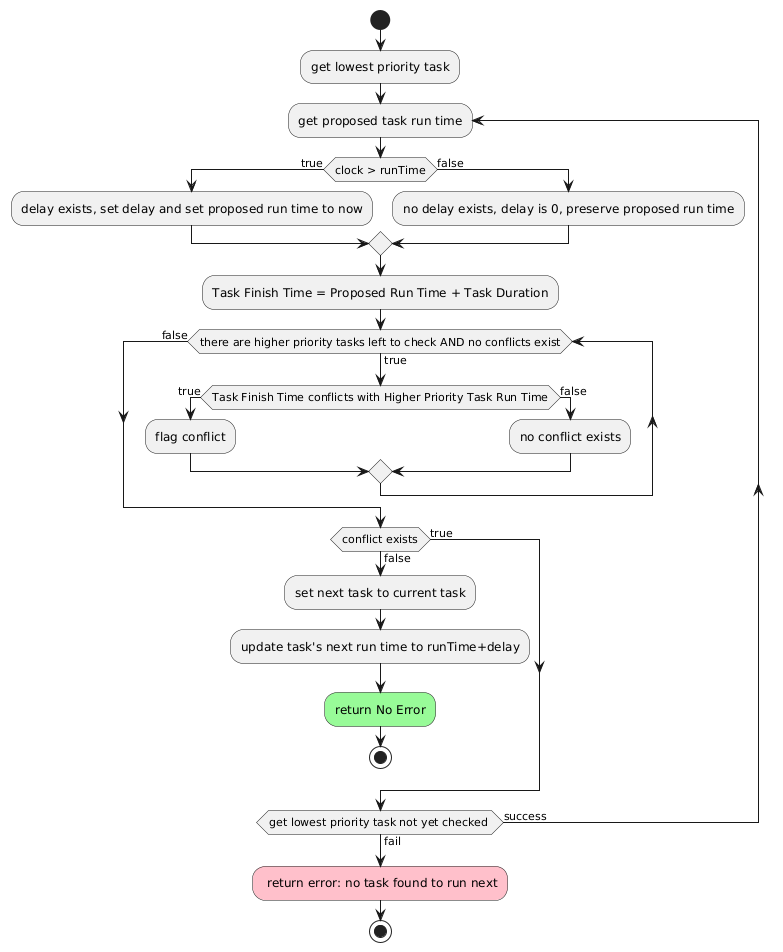
\includegraphics[width=0.6\textwidth]{control_flow.png}
    \caption{Control Flow Diagram of the Algorithm}
    \label{fig:example}
\end{figure}

\section{Scheduler Limitations}
Due to the fact that the SmartFin is a uniprocessor device and the periodicity and length of the tasks, mathematically, it is not possible for all combinations of tasks to run with no shifts in the system. Further, even when allowing for shifts, there exist combinations of tasks in which preserving the frequencies of each task is simply not possible. 


\bibliographystyle{plain} % We choose the "plain" reference style

\bibliography{refs} % Entries are in the refs.bib file
Karger, David, and Cli Stein. Scheduling Algorithms. 1997.

\end{document}

